\documentclass[times, utf8, diplomski]{fer}
\usepackage{booktabs}
\usepackage[croatian]{babel}
\usepackage[utf8]{inputenc}
\usepackage{pdfpages}

\setcounter{secnumdepth}{3}
\setcitestyle{numbers}
\graphicspath{ {./images/} }

\begin{document}

\thesisnumber{1373}

\title{Analiza i usporedba sigurnosnih mehanizama u Internetu stvari}

\author{Filip Ptiček}

\maketitle

% Ispis stranice s napomenom o umetanju izvornika rada. Uklonite naredbu \izvornik ako želite izbaciti tu stranicu.
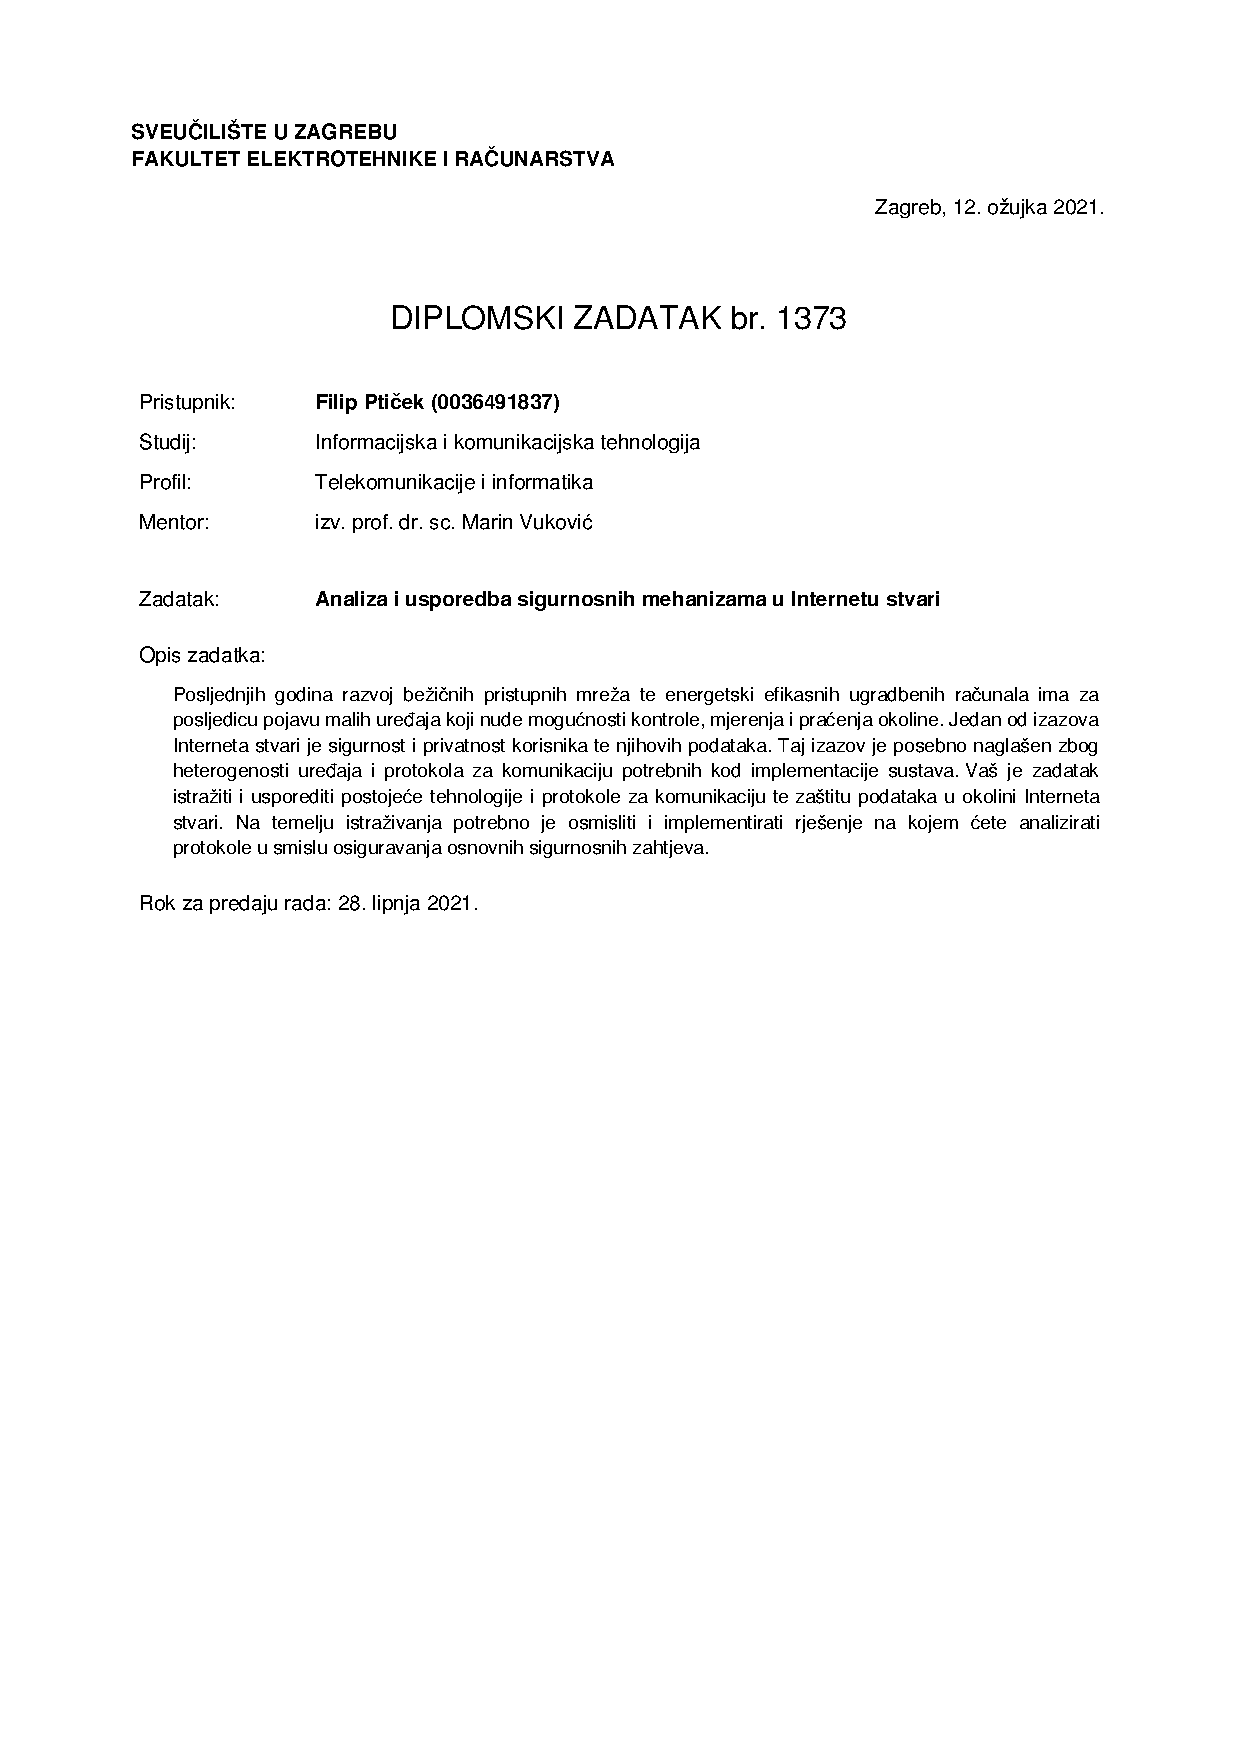
\includepdf[pages=-,fitpaper=true]{zadatak.pdf}

% Dodavanje zahvale ili prazne stranice. Ako ne želite dodati zahvalu, naredbu ostavite radi prazne stranice.
\zahvala{}

\tableofcontents

\chapter{Uvod}
Uvod u rad

\chapter{Internet stvari}

\section{Definicija}
a

\section{Model IoT sustava}
a

\section{Čimbenici u sustavu}
a

\section{Programske platforme}
a

\section{Otvorena pitanja}
a

\subsection{Sigurnost}
a

\subsection{Privatnost}
a

\subsection{Skalabilnost}
a

\subsection{Decentraliziranost}
a

\section{Primjene}
a

\subsection{Područja primjene}
a

\subsection{Zahtijevi sustava s obzirom na primjenu}
a

\section{Trendovi}
a


\chapter{Sigurnosni zahtijevi u Internetu stvari}

\section{OWASP Top 10}
The Open Web Application Security Project® (OWASP) je neprofitna organizacija čiji je cilj napredak i poboljšanje računalne sigurnosti informacijskih sustava. OWASP kroz svoje projekte otvorenog koda vođenih putem razvojne zajednice radi na poboljšanju sigurnosti Interneta.

\emph{OWASP Internet of Things Project} je projekt osmišljen kako bi pomogao proizvođačima, programerima i potrošačima bolji uvid i razumijevanje u sigurnosne probleme vezane uz Internet stvari. Na taj način korisnici u bilo kojem dijelu razvojnog procesa mogu donositi bolje odluke kod razvoja, postavljanja i pristupanja tehnologijama Interneta stvari.\citep{owasp1} 2018. godine izlazi \emph{OWASP IoT Top 10} lista koja reprezentira deset najčešćih ranjivosti Internet stvari sustava. Svih deset sigurnosnih ranjivosti su navedeni u nastavku uz opis sigurnosnih zahtijeva koji bi trebali spriječiti te ranjivosti i sigurnosne propuste. 

\subsection{Slabe, pogodljive ili tvrdo kodirane lozinke}
Prvi navedeni sigurnosni problemi kod Internet stvari sustava su vezni uz lozinke. Kako bi se uređaju moglo pristupiti i naknadno ga konfigurirati, uređaji dolaze s korisničkim računima koji služe korisnicima kako bi ih mogli upariti sa željenim sustavim ili kako bi proizvođač mogao upravljati uređajem u slučaju pomoći korisnicima ili ažuriranja uređaja. Za pristup tom korisničkom računu uređaja je potrebna lozinka koju krajnji korisnik kod prve upotrebe treba postaviti. Navike korisnika su većinom da iskoriste njima dobro poznatu lozinku koju koriste i za svoje druge korisničke račune. Ako napadač dobije pristup jednoj njihovoj lozinci ima i pristup ostalim računima. Na taj način se pristup korištenim uređajima koji imaju isto korisničko ime ili e-mail adresu i lozinku uvelike olakšava. Korisnici imaju i naviku koristiti slabe lozinke koje su vrlo česte i jako lako pamtljive. Tako su neke od najčešće korištenih lozinka jednostavni nizovi numeričkih znakova ili nizovi znakova na tipkovnici poput: 123456, 123456789, qwerty, ili sam engleski prijevod lozinke \engl{password}.\citep{pass1}. Napadi na lozinke se provode putem takozvanih \emph{brute force} napada. Kako je procesna snaga današnjih računala dosegla vrlo visoke brzine računanja, tako se jednostavne i kratke lozinke mogu pogoditi u vrlo kratkom vremenu.

Ovakvi propusti ne zaobilaze ni proizvođače samih sustava i uređaja. Kod proizvodnje proizvođači na uređaje postavljaju iste lozinke za sve uređaje kako bi kod testiranja ispravnosti lakše pristupili istima. Jedan od najboljih pokazatelja takvog pristupa su usmjerivači/modemi telekom operatera za pristup Internetu koji imaju postavljenu istu zadanu lozinku i korisničko ime poput "admin" ili "user" koju krajnji korisnici uređaja nikada ne promjene. Problem se također pojavljuje i u tvrdo kodiranim \engl{hard coded} lozinkama. Proizvođači postave takve lozinke na uređaje kako bi se uređaji mogli nesmetano povezati s vanjskim servisima, kako bi se proizvođači povezli na uređaj zbog otklanjanja pogrešaka ili kao način za vanjsko upravljanje uređaja. Ako napadač ima fizički pristup uređaju on može skenirati memoriju i pomoću raznih alata pronači lozinku spremljenu na samom uređaju. A kako prozivođači najvjerojatnije koriste istu lozinku za sve iste modele uređaja, napadač ima lak način za pristup i ostalim istim uređajima.

Kako bi se spriječila ova vrsta ranjivosti neki od sigurnosnih zahtijeva koji bi se trebali pratiti su sljedeći. Korisnici bi kod prve upotrebe uređaja trebali promjeniti zadanu lozinku koristeći duge, kompleksne i jedinstvene nizove znakova. Najjednostavniji način postići te zahtijeve je korištenjem upravitelja lozinkama. Oni daju mogućnost generiranja lozinki uz mogućnost spremanja istih bez potrebe da korisnik mora pamtiti sve jedinstvene i duge lozinke. Što se tiče zahtijeva sa strane prozivođača, oni bi trebali razriješiti bolje načine upravljanja uređajima kako bi se izbjeglo korištenje istih ili čak tvrdo kodiranih lozinka za pristup uređaju ili vanjskim servisima. Također bi proizvođači trebali upozoriti korisnika kod uspostave uređaja da promijeni zadanu lozinku.

\subsection{Nesigurne mrežne usluge}
Internet stvari uređaji koriste razne mrežne usluge kako bi mogli komunicirati s vanjskim servisima. Kako je moguće pristupiti tim uređajima putem Interneta potrebno je pravilno osigurati sigurnost tih mrežnih usluga koje se izvršavaju. Neautoriziran pristup preko usluga iskorištavajući zadane lozinke, otvorene mrežne priključke te nepravilno podešeni vatrozidi dozvoljavaju napadaču da dobije pristup uređajima i poslužiteljima. Takvi napadi dozvoljavaju izvršavanje malicioznog koda, iskorištavanje uređaja za botnet, krađu podataka ili onesposobljavanje sustava.
%Expand a little bit

Neki od sigurnosnih mjera koje se mogu poduzeti za osiguravanje mrežnih usluga su: \begin{itemize}
    \item korištenje zasebne lokalne mreže za sve pametne uređaje,
    \item spajati uređaje na isključivo sigurne mreže,
    \item instaliranje regularnih softverskih ažuriranja,
    \item isključivanje svih usluga koje pružaju vanjski pristup uređaju,
    \item isključivanje nepotrebnih mrežnih priključaka i usluga,
    \item isključivo korištenje protokola koji koriste enkripciju.
\end{itemize}

\subsection{Nesigurna sučelja ekosustava}
Nesigurna web sučelja, pozadinski API-jevi, servisi u oblaku i mobilna sučelja, koja dozvoljavaju komunikaciju i interakciju s uređajem, čine sveukupni ekosustav Internet stvari. Kompromitacija bilo kojeg dijela sustava može uzrokovati i kompromitaciju cijelokupnog sustava. Ranjivost kod načina autorizacije i autentifikacije između uređaja i poslužitelja ili korisnika mobilnih i web aplikacija i poslužitelja su jedan od vektora napada na sustav. Također nedostatak ili korištenje slabe enkripcije kod komunikacije može uzrokovati da napadač presretne i iskoristi sakupljene informacije za napad. Nedostatak pravilnog filtriranja ulazno/izlaznih podataka može dovesti do napada poput SQL injekcije. Još jedan projekt OWASP organizacije je \emph{OWASP Top 10 Web Application Security Risks} koji nudi popis najčešćih ranjivosti za web i mobilne aplikacije. Nesigurna sučelja ekosustava imaju direktnu poveznicu s tim ranjivostima koje su: \begin{itemize}
    \item injekcije (SQL, NoSQL, OS, LDAP),
    \item neispravna autentifikacija,
    \item izlaganje osjetljivih podataka,
    \item XML External Entities(XXE) napadi,
    \item neispravna autorizacijska kontrola,
    \item pogrešna konfiguracija servisa,
    \item Cross-Site Scripting(XSS),
    \item nesigurna deserijalizacija podataka,
    \item korištenje bibilioteka i komponenta s poznatim sigurnosnim ranjivostima,
    \item nedovoljno korištenje logova i praćenja sustava.\citep{owasp2}
\end{itemize}

Pravilno podešavanje autorizacije i autentifikacije korisnika, ali i uređaja je najvažniji način osiguravanja raznih sučelja ekosustava. Filtriranje ulaznih i izlaznih podataka spriječava napade injekcijom, pravilno podešavanje poslužitelja da koriste pravilne enkripcijske načine komunikacije dozvoljavaju privatnu i sigurnu komunikaciju. Kroz cijeli ekosustav je potrebno i uspostava logiranja i praćenja sustava kako bi se na vrijeme otkrili nepravilna ponašanja unutar samog sustava.

\subsection{Nedostatak mehanizama za sigurnosna ažuriranja}
Kroz vrijeme, za programska rješenja koja se trenutno koriste na uređaju će se pronači ranjivosti. Kako bi se na vrijeme i jednostavnim putem mogli spriječiti napadi koji iskorištavaju te ranjivosti potrebna su nam softverska ažuriranja, kao i ažuriranja samog ugrađenog programa \engl{firmware} uređaja. Ako ne postoji način kojim dovodimo takva sigurnosna ažuriranja na uređaj postoji rizik za kompromitacijom uređaja. Također ako su i implementirani načini sigurnosnih ažuriranja, potrebno je pridodati pažnju na način te implementacije ažuriranja. Ako se ne provjeravaju digitalni potpisi izvora ažuriranja, moguće je na uređaj poslati maliciozno ažuriranje koje će kompromitirati uređaj. Potrebno je i koristiti sigurne načine prijenosa tih ažuriranja poput enkripcije upotrebljavanog komunikacijskog kanala. 

Trenutnim trendom brzog razvoja novih uređaja, prozivođači često ne daju dovoljno dugi period sigurnosnih ažuriranja. Tako će se desiti da proizvod nakon manje od dvije godine prestane dobivati ažuriranja te će pasti odluka na korisnika o tome hoće li kupiti novi uređaj ili riskirati kompromitaciju istog. Najbolji pokazatelj toga su pametni telefoni od kojih većina tijekom svog perioda upotrebe dobije samo nekoliko sigurnosnih ažuriranja prije nego bude depricirana od strane prozivođača.

Kako bi se uređaji zaštili od budućih napada zbog novootkrivenih sigrunosnih propusta potrebno je pružati korisnicima uređaja nuditi dugotrajna i česta sigurnosna ažuriranja. Prijenos ažuriranja je neophodno prenositi putem sigurnih komunikacijskih kanal koji su enkriptirani. Ažuriranjima koja su dostigla na uređaj je potrebno validirati izvor, provjeriti odgovara li digitalni potpis izvoru od kojeg bi trebalo stići ažuriranje. Također je potrebno i validirati samo ažuriranje kako bi se izbjeglo moguće umetanje malicioznog koda.

\subsection{Upotreba nesigurnih ili zastarijelih komponenti}
Nadovezano na nedostatak mehanizama za sigurnosno ažuriranje, peta po redu od sigurnosnih propusta je upotreba nesigurnih ili zastarijelih komponenti. Mnogi sustavi Internet stvari kao dio svojeg programskog riješenja sadrže otvoreni kod koji održava zajednica koja nije direktno povezana s proizvođačem. Kada se otkrije ranjivost na nekom od korištenih otvorenih rješenja proizvođač ili čeka na sigurnosnu zakrpu, ili u najboljem slučaju će sam riješiti sigurnosni propust te ga javno objaviti kako bi doprinjeo razvoju otvorenog rješenja. Nakon što sigurnosna zakrpa bude razvijena potrebno je ažurirati sve uređaje ili dijelove sustava koji su ugroženi od tog sigurnosnog propust. 

Ako govorimo o Internetu stvari u proizvođačkoj industriji, takozvanoj Industriji 4.0, upotreba zastarijele programske podrške, koja je potrebna zbog jako specifičnih uređaja za prozivodnju, čija zadnja verzija zna datirati i više od deset godina nije rijetka. Uvođenjem takvih uređaja u sustave Interneta stvari također utječe na sigurnost i integritet cijelokupnog sustava te ugrožavanje jednog uređaja može dovesti do napada na cijelog lanca opskrbe. Kod upotrebe gotovih proizvoda poput senzora, videokamera ili pametne rasvijete te integracijom istih u postojeći sustav također treba obratiti pozornost na dostupnost sigurnosnih ažuriranja te stanje uređaja poput je li proizvođač još uvijek nudi sigurnosnu podršku.

Kod planiranja razvoja Internet stvari sustava potrebno je uzeti u obzir trenutno, a i buduće stanje razvojne i sigurnosne podrške vanjske programske potpore i komponenti sustava. Najbolji način za spriječavanje sigurnosnih propusta je korištenje vlastito razvijene programske potpore ili korištenje dobro podržanih vanjskih biblioteka otvorenog koda s jakom i aktivnom razvojnom zajednicom. Uporeba zastarijelih uređaja bez sigurnosne podrške proizvođača ili potporom koja uskoro dotiže krajnji period \engl{end of life} je potrebno izbjegavati. Nakon puštanja sustava u produkciju nadziranje i praćenje vijesti vezanih uz sigurnosne propuste upotrebljenih komponenti i programske podrške je važno kako bi se na vrijeme moglo spriječiti kompromitacija sustava. Sve ovo nije moguće ako bilo koji dio ustava nema implementirane mehanizme za sigurnosna ažuriranja. Ako neka od komponenti dostigne svoj krajnjio period ažuriranja potrebno je tu komponentu ukloniti i zamijeniti ju drugom čija sigurnosna ažuriranja još uvijek su podržana.  

\subsection{Nedovoljna zaštita privatnosti}
Uloga Interneta stvari je djelom prikupljanje različitih podataka i mjerenja. Neki od tih podataka su osobne prirode za korisnika poput: medicinskih podataka ili zvukovnih i video zapisa. Kompromitacija takvih privatnih podataka može negativno utjecati na sigurnost korisnika. Prostor na kojem se privatnost korisnika može narušiti je od samog uređaja koji prikuplja podatke, do komunikacijskih kanala preko kojih se podaci šalju do samih krajnjih servisa koji primaju i obrađuju te podatke, a zatim ih spremaju u baze podataka na poslužiteljma. Nedovoljna zaštita privatnosti je zapravo rezultat svih ostalih nabrojanih sigurnosnih ranjivosti nabrojanih u ovom odjeljku. 

Za očuvanje privatnosti korisnika i načine obrade podataka korisnika u Europskoj uniji postoji uredba donešena od strane Europske unije pod nazivom \emph{Opća uredba o zaštiti podataka(GDPR) (EU) 2016/679}\citep{GDPR}. Cilj uredbe je omogućiti građanima Europske unije veću kontrolu i uvid u podatke koji se prikupljaju. Na taj način građani mogu tražiti brisanje svojih podataka i povećava se odgovornost pravnih osoba koje te podatke prikupljaju. Odgovornost se postiže mogućim nametnutim sankcijama, ako se utvrdi povreda podataka građana. Prikupljanje podataka je moguće uz izrazitu privolu građana korisnika čime se zabranjuje bilo kakvo prikupljanje podataka bez pristanka. 

Enkripcija komunikacijskih kanal nekada ne osigurava i privatnost korisnika. Kako bi pametni uređaji mogli komunicirati s krajnjim poslužiteljima, koji mogu mijenjati svoju odredišnu adresu, koriste se domenska imena. Za razlučivanje tih adresa u brojčanje IP adrese koristi se protokol DNS\engl{Domain Name System}. Kada uređaji rade DNS upite u sadržaju upita se prikazuje i domena upita u nekriptiranom formatu. Na taj način napadač može iz konteksta upita zaključiti koji uređaji proizvođača se nalaze u mreži korisnika. Za neke uređaje je moguće zaključiti i sam tip, a ne samo proizvođač. U sljedećoj tablici možemo vidjeti uređaje i DNS upite koje proizvode:
\begin{table}[h]
    \centering
    \begin{tabular}{c || c } 
    \textbf{Uređaj} & \textbf{DNS upiti} \\
    \hline\hline
    Nest Security Camera & nexus.dropcam.com \\
     & oculus519-vir.dropcam.com \\
     & pool.ntp.org \\
    \hline
    Amazon Echo & ash2-accesspoint-a92.ap.spotify.com \\ 
     & audio-ec.spotify.com \\ 
     & device-metrics-us.amazon.com \\ 
     & ntp.amazon.com \\ 
     & pindorama.amazon.com \\ 
     & softwareupdates.amazon.com \\
    \end{tabular}
    \caption{Primjer DNS upita napravljenih od strane uređaja \citep{Apthorpe2017May}}
    \label{tab:confusion}
\end{table} \\
Još jedan način na koji se može zaključiti o trenutnoj aktivnosti korisnika u vlastitoj mreži je i broj paketa koji se šalje u danom trenutku van mreže i njihova periodičnost. Ako se radi o uređaju koji ima mogućnosti virtualnog asistenta moguće je imati uvid u to kada je korisnik imao interakciju s uređajem. Također kod uređaja koji prate spavanje korisnika se broj razmijenjenih paketa drastično poveća kada korisnik spava.\citep{Apthorpe2017May}

Kako najbolje očuvati privatnost korisnika je pitanje s kojim još uvijek mnogi prozivođači imaju problema. To se očituje u ostalim navedenim sigurnosnim propustima u ovom odjeljku. Zakonskim regulativama postiže se veća svijest o bitnosti zaštite podataka te se samim time proizvođači tjeraju na bolje prakse za očuvanjem podataka. Neki od osnovnih načina zaštite korisničkih podataka su: 
\begin{itemize}
    \item enkripcija podataka u svakom aspektu sustava,
    \item prikupljanje samo nužnih podataka,
    \item anonimiziranje korisnika,
    \item bolja kontrola i uvid u podatke za korisnike.
\end{itemize}

\subsection{Nesigurni prijenos i pohrana podataka}
Podaci koji nisu kriptirani moguće je vrlo lako iščitati. Kriptografijom se postiže sigurnost i privatnost podataka. Kako bi se to postiglo podatke je potrebno kriptirati u svokm koraku njihova nastajanja, prijenosa, obrade i spremanja. Korištenje samih kriptografskih alogritama ne rezultira uvijek i zaštitom podataka. Neki kriptografski algoritmi koriste ključeve nedovoljne dužine i kao takve je potrebno malo vremena da se dešifriraju. Najveći sigurnosni propusti u nedavnoj povijesti povezani su dirketno s nedovoljnim kriptografskim algoritmima ili općenitim nedostatkom šifriranja čime su ugroženi osobni podaci i lozinke korisnika.\citep{DataBreaches} Pozornost se treba posvetiti i kontroli pristupa podacima kako neautorizirani korisnici ne bi mogli pristupiti nedozvoljenim podacima. 

Osnovni sigurnosni zahtijevi koji bi se trebali osigurati su: \begin{itemize}
    \item šifriranje podataka,
    \item pravilno korištenje PKI-a \engl{public key infrastructure},
    \item kontrola pristupa podacima,
    \item korištenje sigurnih protokola za prijenos podataka,
    \item provjera korištenih kriptografskih algoritama za ranjivosti,
    \item korištenje dugih kriptografskih ključeva.
\end{itemize}     

\subsection{Nedostatak mogućnosti upravljanja uređajima}
a

\subsection{Nesigurne zadane postavke}
a

\subsection{Nedostatak fizičke sigurnosti}
a

\section{Primjeri sigurnosnih napada i propusta}
a

\chapter{Analiza i usporedba protokola}

\section{IoT stack}
Iot stack

\section{Fizički sloj}
Senzori

\subsection{Analiza uređaja}
Uređaji

\subsubsection{Senzori s komunikacijskim modulom}
a

\subsubsection{Pristupni uređaji}
a

\subsection{Usporedba sigurnosnih mehanizama i primjena}
a

\section{Sloj podatkovne poveznice}
a

\subsection{Analiza tehnologije protokola}%Promjeni protokola u tehnologije
a

\subsubsection{WiFi}
a

\subsubsection{BLE}
a

\subsubsection{RFID\textbackslash NFC}
a

\subsubsection{ZigBee}
a

\subsubsection{LTE}
a

\subsubsection{SigFox}
a

\subsubsection{LoRaWan}
a

\subsection{Usporedba sigurnosnih mehanizama i primjena}
a

\section{Mrežni sloj}
a

\subsection{Analiza protokola}
Neki protokoli

\subsubsection{IPv4}
a

\subsubsection{IPv6}
a

\subsection{Usporedba sigurnosnih mehanizama i primjena}
a

\section{Transportni sloj}
a

\subsection{Usporedba primjena protokola}
a

\section{Aplikacijski sloj}
a

\subsection{Analiza protokola}
a

\subsubsection{HTTP/S}
a

\subsubsection{COAP}
a

\subsubsection{MQTT}
a

\subsection{Usporedba sigurnosnih mehanizama i primjena}
a

\chapter{Sustav za praćenje tjelesne temperature}

\section{Arhitektura sustava}
a

\section{Korišteni razvojni alati i uređaji}
a

\section{Opis rada sustava}
a

\section{Sigurnosna analiza sustava}
a


\chapter{Zaključak}
Zaključak.

\bibliographystyle{fer}
\bibliography{literatura}
\listoffigures
\listoftables

\begin{sazetak}
Sažetak na hrvatskom jeziku.

\kljucnerijeci{Ključne riječi, odvojene zarezima.}
\end{sazetak}

% TODO: Navedite naslov na engleskom jeziku.
\engtitle{Title}
\begin{abstract}
Abstract.

\keywords{Keywords.}
\end{abstract}

\end{document}